\documentclass[11pt, oneside]{article}
\usepackage{geometry}
\usepackage{amssymb,amsmath,amsthm}
\usepackage{amsfonts,bm}
\usepackage{caption,subcaption}
\usepackage{graphicx}
\usepackage{listings}

\title{sche\_simulator Code Guidance}
\author{Yubo Feng}

\geometry{left=2.5cm,right=2.5cm,top=1.5cm,bottom=2.5cm}
\setlength{\parindent}{0pt}
\begin{document}
\maketitle
\textbf{Abstract:} sche\_simulator is a real time simulator framework consisted of basic components including task set generator, scheduler and energy model. The design purpose of this simulator is to proved a easy programming framework to help researcher to implement, analysis and verify various schedule algorithm performance as well as energy costing. 

\section{Design for each module}
\subsection{Introduction}
The simulator is consists of four part: ts (taskset generator), sche (scheduler), em (energy model) (I keep using those abbr in code variable name) and exp(experiment). Each of those parts is a class, and all member variables (except error code) are kept in private, since I want to make each module as isolated as possible. You only need to change the part that matters for you, and you needn't worry about other module. \textbf{The principle of whole framework focuses on reusable and structure, but not performance nor detail implementation of each algorithm.} For each module, I will describe it in following aspects:
\begin{enumerate}
\item \textbf{Design principle}, describing the major structure of current module
\item \textbf{key structure and design concern}, describing design concern like why this component is designed like this
\item \textbf{example}, describing how to use this module and where to see reference code
\end{enumerate}
Sometimes one or two part will be miss, not because it is not important, but it has already combined in previous paragraph.

\subsection{TaskSet Generator}
\subsubsection{Design principle}
TaskSet generator is used for generate specific number of tasks in some kind of distribution, for example, we want to generate 20 tasks for each period range is between 10 and 100, and computational time is normal distribution between 10 and 100. According to this requirements, the class is defined as below: \\

A simple model is used to define task structure: \textit{task\_tpl}: it just includes c, p and u, while for a group of tasks, it defines as vector in class TaskSet: \textit{\_tasks}. The properties of TaskSet including distribution of computation time and period, lcm, period range, total utilization, probability range. All those properties are regarded as task set properties, so there are set of variables inside the class to record their settings, for example like \textit{\_dis\_c}, \textit{\_cur\_prob\_range}, \textit{\_lcm}, while here are some methods to set or get value of those variables, for example like \textit{get\_lcm()}, etc.. \\

Currently, only distributions of uniform and normal distribution is supported, both methods are implemented in MathHelper class: if you want to add your own distribution type, please look at \textit{MathHelper::dis\_reg()}: just like register, the MathHelper cannot detect what kind of distribution it has, so it will call \textit{MathHelper::dis\_reg()} to add all the methods it has to member variable: \textit{\_dis\_set}, \textit{\_dis\_map}, only after this, MathHelper will know what kind of distribution it has, so it could call correspond method to generate random number. \\

\textit{\textbf{Note 1}: the distribution that current MathHelper has comes from C++ STL library, \\see description in \underline{http://www.cplusplus.com/reference/random/}}\\
\textit{\textbf{Note 2}: in order to support different distribution selection according to input string, function pointer is used, variable \textit{MathHelper::gen\_rd\_dis} is a functional pointer point to input determined random number generator. }\\

After setting all type of parameters for current task set, call \textit{TaskSet::gen\_task\_set()} will generate according to setting, and \textit{TaskSet::get\_task\_set()} will return this group of tasks, later, scheduler will use this task set to do schedule algorithm. Actually, the task set will not give you a full utilization task set, by this means: the task set will contain specific number of tasks, but total utilization is total random. If you want to have a special task set that could generate targeted total utilization, you have to implement your own and call in your function.

\subsection{Scheduler}
\subsubsection{design principle}
Scheduler class is where basic scheduler is. I am not intended to implement specific scheduling algorithm, but try to give a abstract model. Considering: regardless of which kind of scheduling algorithm, all it needs is a task set, energy model (optional) (when task set mentioned, it also includes lcm, distribution, all kind of properties); regardless of which kind of scheduling algorithm, all it generate is a scheduling table (which task should be there for specific time slot) and speed table (gives for each time slot, what speed should be here). Therefore, a general scheduler is required which is a high abstracted scheduler that could provide uniform interface for task set generator and energy model. For software engineer purpose, if such abstract scheduler exists, then each model is highly isolated, and it is easy to debug and handle. That is where class \textbf{Scheduler} come from. \\

Again, class Scheduler is a base class, you SHOULD inherent from this base class and implemented your own scheduler algorithm; but from outside view, it provided two methods: \textit{init\_sche} and \textit{exec\_sche} that used for init scheduler and run simulator. For \textit{init\_sche}, currently, we just reset all configuration and clear the speed table, scheduling table; for \textit{exec\_sche}, it will first clone one task set and then pad this task set to 100\% utilization, and then call a private method called \textit{exec\_full\_util\_sche}, what this method did is that: it will take a full utilization task set and then schedule on this full utilization task set. After the scheduling, the scheduler will call mask\_sche\_table to remove padding tasks, for example, the original task set is 18.25\%, 20 tasks will be contained; \textit{exec\_sche} will first pad, say, 3 more tasks, in order to make current task set to be 19\% utilization (now new task set will have 23 tasks). Then it will call \textit{exec\_full\_util\_sche} to schedule; after schedule done, \textit{exec\_sche} will remove tasks 20 - 12 from speed table and schedule table where correspond value in speed table will be set to min speed of current core based on energy model, while value in schedule table will be set to -1 (default value). So the final output will be schedule table and speed table for original task set. \\

\textit{\textbf{Note}:The reason why \textit{exec\_sche} use this type of method lies in historical reason: source code for algorithms Bfair and Pfair are both build under assumption that input task set utilization is 100\%. I don't want to touch this part of source code, so I build this type of mechanism in order to match these two type of algorithms. Moreover, I implemented \textbf{dvfs\_bfair\_scheduler}, in this scheduler, you can find what to do if you want to abandon this mechanism and build a scheduler that accept any task set as input and schedule them. }

\subsubsection{key structure and design concern}
In general, the scheduler will accept three parameters as constructor: \textbf{stop\_point}, which is for termination purpose (we don't want to this simulator run too long time, so use this parameter to stop simulator at some time point); \textbf{num\_proc}, which is number of processors, in some energy sensitive scheduler, the more processor, maybe the more energy saving; \textbf{em}, which is energy model, if the algorithm do not have any energy concern, then set this parameter to \textit{nullptr} is sufficient. These three parameters are regarded as basic properties, so in this sense, a bfair scheduler with $stop\_point=1000$, is different with bfair scheduler with $stop\_point=100$. Keep this in mind: scheduler is related to, but relative isolated with corresponding algorithm. The reason why design like this is for experiments purpose, since we may want to compare same schedulers with different energy model or different schedulers with same energy model.\\

Here is some comments on this part: \\
1) for some scheduler, it may require different number of processors as input, while some may require different energy model as input; in order to meet all those requirements, some rules should be followed:
\begin{itemize}
%default
\item in default setting, assumption is that we want to just test 1000 time units, while no particular energy model is required, and no particular number of processors are required to be tested. So the default input is $<1000, ts\to get\_min\_core(), nullptr>$, so this means that if you want to test if one algorithm is correct or not, just set number of processor as min cores, and energy model is nullptr will be fine.
%min core inequation
\item if there is any requirement to use any kind of energy model and test if algorithm could schedule tasks on multiprocessors, so for any input to \textit{exec\_sche}, at least one condition should be follow: \textit{\# of min core of task set $\leq$ \# of cores that energy model provided $\leq$ \# of cores scheduler use}. For example, in energy model, 16 cores are provided, while for some task set, it required at least 7 processors, so if \# of cores as input of scheduler is 3, then error will occur, since it is impossible to schedule; \# of cores as input of scheduler at least is 7(use min cores) but at most 16 (use all processors). For some input: if in energy model, 5 cores are provided, while for some task set, it required at least 7 processors, then there is no algorithm could schedule, so there will be error. 
%config issue
\item for configuration of simulator, there is some setting issue should be noticed, which will be described in experiment chapter.
\end{itemize}

2) if you want to start with your own scheduler, here is basic stuff: 
\begin{itemize}
%build file
\item create a .h file include header \textit{sched.h}, build a class that inherent from class Scheduler
%implement scheduler algorithm
\item if you need info for each task when your scheduler works, then define this special struct within the class inherent from \textit{task\_tpl} (aka, task template) (notice: this means inherent from a structure in grammar perspective)
\item create a .cpp file and implement your own scheduling algorithm, here are two approaches for developer to choose: if you feel that it is comfortable to write down your algorithm for 100\% utilization task set, then what you need to do is just overload method \textit{exec\_full\_util\_sche} and implement this method by taking care of stop\_point, num\_proc, em; otherwise, you should overload methods \textit{init\_sche} and \textit{exec\_sche} then implement both of those methods. \\
\footnotesize{\textit{\textbf{Note}: In previous situation, you needn't consider what will happen for task set that utilization is less than 100\%, but you have to implement algorithm deal with 100\% utilization; in second situation, you have to deal with this situation and take care of it by your own but you get more degree of freedom. There is no recommendation for developer to use which kind of method, it ups to developer.}}
%check valid shedule method
\item currently, method \textit{check\_val\_sche} just includes conflict check (for each time slot, there is no conflict for tasks) and allocation check (if certain task gets sufficient computation time allocation within each period). If you have particular check condition, then overload and implement your own \textit{check\_val\_sche} method. If you choose to use second approach in scheduler, then don't forget to call \textit{check\_val\_sche} when you implement your scheduler.
%test and configuration
\item write down test code in current .cpp file, and test it in main function or local file. After this, when you make sure your algorithm is correct, then extend experiment class and do experiments as your wish to collect data. (\footnotesize{\textit{\textbf{Note}: you can find how to extend config file and experiment class in following chapter.}})
\end{itemize}

\subsubsection{examples}
\begin{enumerate}
\item Bfair scheduler: \\
Bfair scheduler implementation is a good example to illustrate how to implement a simple scheduler: scheduler bfair is implemented in file sche\_bfair.h and sche\_bfair.cpp; this algorithm do not require any energy model, so in this scheduler, just method \textit{exec\_full\_util\_sche} is implemented using first approach; since this algorithm do not need other kind of validation check except conflict check and allocation check, so there is no necessary to overload \textit{check\_val\_sche}. Finally you can test the code within this file, the test code could be found in the bottom of that .cpp file.
\item dvfs\_bfair algorithm:\\
Bfair scheduler implementation is a good example to illustrate how to implement a scheduler that take energy model into consideration: scheduler dvfs\_bfair implemented in file scheduler dvfs\_bfair.h and scheduler dvfs\_bfair.cpp. For dvfs\_bfair algorithm, it requires to know basic info for energy model, and it will deal with the tasks case by case. In this situation, the implementation of dvfs\_bfair algorithm has more work to do than bfair : first, it has to inherent and implement \textit{init\_sche} and \textit{exec\_sche}, since dvfs\_bfair does not require utilization of tasks, so we do not need to implement \textit{exec\_full\_util\_sche} (however, in perspective of c++, if you call this method in your code, you still can get a value! this is because this is a virtual function). After this, since we know that the only part should be checked is the tasks after kth tasks, so the \textit{check\_val\_sche} needed to reimplement as shown in class implementation. This algorithm shows how to implement scheduler by using second approach.
\end{enumerate}

\subsection{Energy Model}
\subsubsection{Calculate Energy}
There are different kind of energy models, in current energy model, it only support square model, which is $E = f^2\times t$, where E is energy cost, f is processor frequency and t is time accumulated. So, if a processor has different frequency in different time, then we will have $E_{total} = f_1^2t_1 + f^2t_2 + ... + f_n^2t_n$ to calculate energy cost, which means the processor run $t_1$ times by frequency $f_1$ totally, run $t_2$ times by frequency $f_2$ totally, and so on so forth. ($t_1$, $t_2$... all is accumulate time.). In this model, we do not consider static energy, but only dynamic energy.

\subsubsection{key structure and design concern}
Energy model has one important member variable: \_proc\_freq, which is a 2 dimension vector; first dimension represent processor, while second dimension represents discrete speeds that this processor has. For example, \_proc\_freq = [[0.5, 3.9], [1.0, 1.5, 2.0], [4.5]], this means current energy model is: three processors, first processor has two level of speed, 0.5GHz and 3.9GHz; second processor has 1.0GHz, 1.5GHz and 2.0GHz, for last processor, it just one kind of speed, 4.5GHz. By default, the speeds for each processor are sorted in increasing order. Energy model will read configuration file to get all those speed vector, see more details in experiment section. Just one remind: if you do not provide any speed config, then if you try to create a object of energy model in program, you still can, but you will "create" a simple model which for all processors, minimum speed is 0.0GHz, while maximum speed is 1GHz.\\

When energy model is used as input for some scheduler, we usually use method \textit{get\_proc\_freq} to get speed vector, and then use it to be some info in scheduler. So you can regard energy model is type of outside information: imagining it is property of some machine, and  your scheduler will schedule task set in this machine. So it is restricted defined which is also provided to be used by scheduler. After scheduler terminate and output correspond schedule table and speed table, all analysis for speed will occur according to those two table. Again, run analysis is meaningful only after schedule is done. For example, in the beginning, a task set is generated, then you could use dvfs\_bfair to schedule; after scheduling, call cal schedule cost to get analysis while use output of scheduler as input. After this, call different methods in energy model to get different aspects of current results.\\

For discrete frequency and continues frequency: it totally depends on developer, developer should know what current model is. No mater what kind of frequency model you choose, finally the speed in time slot should be record in speed table and final energy cost calculation will totally depend on this table. So, in extreme case, in perspective of developer, you can just create some kind of model while never use it as long as you know this will cause no trouble in your algorithm.\\

For future usage, if you want to implement your own energy model, you can simply inherent from energy and implement your own energy model, in this way, nothing in previous module is needed to modified.


\subsubsection{examples}
Here in experiment.cpp, method \textit{run} implements a simple demo program in order to show how to use config file to set config for a experiment and get result. You can find more details in this method.\\

\subsection{Experiment and configuration}
\subsubsection{design principle}
Experiment class is not main module for this simulator. But quite like a "shell" for simulator, since the purpose for designing this module is for user perspective: customizing experiment and execution. The main purpose of experiment class is read configuration file, get basic configuration setting and customize a particular simulator instance according to user's configuration, then run simulator and get results.

\subsubsection{key structure and design concern}
Configuration file is written in grammar defined in \textit{libconfig} which is a open source library (see more details and how to use this lib in \underline{http://www.hyperrealm.com/libconfig/}). \textbf{One type of configuration will map to one kind of experiment class.} So, how to define one kind of configuration decides how to define your experiment class and vice versa. When implementing experiment class, you will create simulator pipeline by your own according to your configuration file input. \\
\textit{\textbf{Note}: in \textit{libconfig}, it is restricted to distinguish 0 and 0.0: former represent integer zero, and the latter represent float format zero}\\

The reason why design like this lies in isolation of perspective of developer and user. Developer will focus on implement details of algorithm, while, when comes to experiments, it will more likely a user perspective, but not developer. In another word, though there will be a lot of different in processing of algorithm, but there will always similar when comes to experiments. From my own experience, sometimes, it requires a lot of redundancy work in implement experiment code and configure them for different experiment requirement. So, if we can isolate experiment and development process, this will save researcher a lot of time.\\

In previous development of simulator, author of the simulators always manage the experiment by themselves and write down everything. This is a curse for reusable code. If we use c/c++ to implement experiment schema, it will be hard to maintain and use for future experiment and other researcher, since other people, sometimes even author himself will forget what is written. But if we use script language like shell scripts or python, we may not take advantage of execution speed: it is costly to create process. So, to find a balance point, considering for user to customize their own experiments, experiment class is created. \\

Experiment class is like a shell, it controls the process of how simulator goes: for example, after you implement this type of algorithm, then when you try to test it, you could create a experiment class for this certain scheduling algorithm, then config it and test it; later, if you want to compare this algorithm with some other algorithm, you could create a new experiment class that could let you combine both object algorithms' experiment classes, and use config file to determine what to do for both of them. So, in this sense, experiment class acts quite like a "compiler", it compiles configuration file and gives your correspond simulator under this type of configuration. \\

In current design, two method are critical: constructor \textit{experiments} and method \textit{run}. Input for constructor is a path to configure file, when create instance of current class, it will read from configuration file and use \textit{libconfig} to parse this .cfg file and store correspond parameters. Then in method \textit{run}, all those parameters read from file, stored in member variables, will be manipulated to create a simulator instance and execute it, and finally output result. \\


\subsubsection{example}
How this class works highly depend on the design of configuration file and what type of experiment you want to do, in files experiments.h and experiments.cpp, one example is given in order to illustrate how to create this type of class. \\

In this example, all settings will be load from configuration file and stored in member variables. In the beginning, the experiment constructor will "register" all current scheduler algorithm into member variable \textit{\_schduler\_map}, basically, \textit{\_schduler\_map} is a hash table, map from scheduler algorithm to a integer. Then, it will keep loading the file, and get parameters for each components, for example, distribution of computational time, \# of tasks in task set, speed vector and so on. \\

Then, method \textit{run} will create correspond scheduler according to configured scheduling algorithm, task set will be created, and energy model will be created, finally, \textit{init\_sche} and \textit{exec\_sche} methods will be called, and result will be shown in the std output. If you read method \textit{run}, basic the whole method is implemented in this way. Moreover, in main function, actually, it just create the experiment instance and execute it. As one can see, even you have a lot of experiment to run, but you can combine them and show then in a very clear and structure way.\\

 \textit{\textbf{Note}}: in current .cfg file, if there is no configuration for proc\_speeds (no such item in .cfg file) and num\_proc is set to -1, then current implementation will set input parameter of num\_proc for scheduler to minimum \# of processors required for current task set. However, if no configuration for proc\_speeds and num\_proc is not -1, then, when call \textit{exec\_sche}, it will check if num\_proc $\leq$ min \# of cores, if it fails, the current task will be rejected. Moreover, if there is configuration for proc\_speeds and num\_proc is not -1, then it will check if \textit{\# of min core of task set $\leq$ \# of cores that energy model provided $\leq$ \# of cores scheduler use } just as described before.
 
\section{Structure of simulator}
\begin{figure}[h]
\centering
	\begin{subfigure}[h]{0.5\textwidth}
		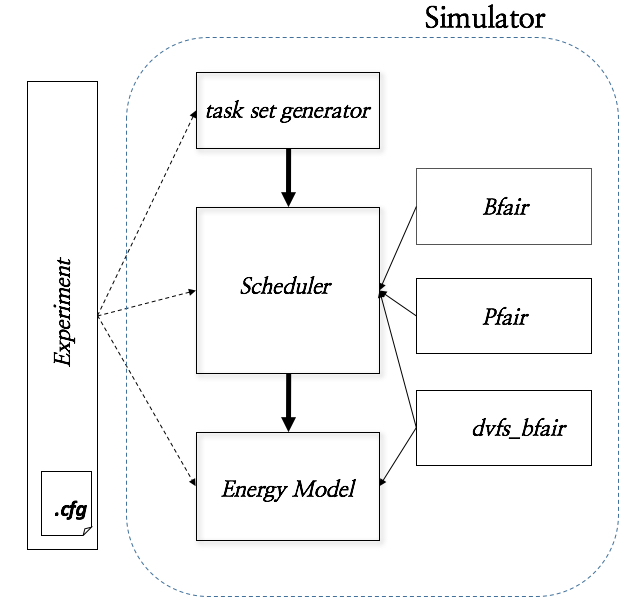
\includegraphics[width=\textwidth]{figure}
	\end{subfigure}%
\caption{Structure of Simulator}
\label{struct of simulator}
\end{figure}

Figure.1 shows the basic structure of simulator, as it indicates, simulator itself includes task set generator, scheduler and Energy Model three parts, and experiment component in outside of the simulator, in order to set configuration for each component. The black width arrow shows the data flow among components. Dotted line shows control (configuration) for each component. Thin arrow shows the inherent relationship. 

\section*{Updates}
5/3/2016 by Yubo Feng : this document is created.













\end{document}
